\documentclass[a4paper,twoside,openright,11pt]{book}

\usepackage{setspace}

\usepackage{amsmath}
\usepackage{amssymb}

\usepackage{array}
\usepackage{amsthm}
\usepackage{amsfonts}
\usepackage{mathtools}
\usepackage{makeidx}
\usepackage[pdftex]{graphicx}
\usepackage{url}
\usepackage{epigraph}
\usepackage{hyperref}

\usepackage{fancyhdr}

\usepackage{hyperref}

\usepackage{type1cm}
\usepackage{lettrine}

\usepackage{color}
\usepackage{colortbl}
\usepackage{placeins}

\usepackage{multirow}

\usepackage{titlesec}
\titleformat{\chapter}[display]
{\normalfont\bfseries\filcenter}
{\LARGE\thechapter}
{1ex}
{\titlerule[2pt]
\vspace{2ex}%
\LARGE}
[\vspace{1ex}%
{\titlerule[2pt]}]

\usepackage{algorithmic, algorithm}

\usepackage[squaren, Gray, cdot]{SIunits}

\usepackage{rotating}

\usepackage{tikz, pgfplots}
\usepackage{tikz-qtree}

\usetikzlibrary{patterns}

\renewcommand{\algorithmicrequire}{\textbf{Input:}}
\renewcommand{\algorithmicensure}{\textbf{Output:}}

% Setup pdf meta-data.
\hypersetup{ % Modifiez la valeur des champs suivants
pdfauthor = {Antonio El Khoury},
pdftitle = {FIXME},
pdfsubject = {FIXME},
pdfkeywords = {Motion Planning, Optimal Control, Humanoid Robot},
pdfcreator = {Antonio El Khoury},
pdfproducer = {Antonio El Khoury}
}

% Customize chapter head.
\makeatletter
\renewcommand\chapter{\if@openright\cleardoublepage\else\clearpage\fi
                    \thispagestyle{empty}%
                    \global\@topnum\z@
                    \@afterindentfalse
                    \secdef\@chapter\@schapter}
\def\@makechapterhead#1{%
  \vspace*{50\p@}%
  {\parindent \z@ \raggedright \normalfont
    \ifnum \c@secnumdepth >\m@ne
      \if@mainmatter
        \Huge\bfseries\thechapter\enspace
      \fi
    \fi
    \Huge \bfseries #1\par\nobreak
    \vskip 40\p@
  }}
\makeatother

\newcommand\vect[1]{\textbf{#1}}
\newcommand\moment[2]{{\cal M}_{#2}^{#1}}
\def\crossprod{\times}

\def\vi{\vect{v}_{i}}
\def\vG{\vect{v}_{G}}
\def\gammai{\gamma_{i}}
\def\gammaG{\gamma_{G}}

% Enforce math style.
\everymath{\displaystyle}

% Generate index.
\makeindex

% Please fancyhdr.
\pagestyle{headings}
\setlength{\headheight}{25pt}

% Align bibliography left and add some padding
\makeatletter
\renewcommand{\@biblabel}[1]{[#1]\hfill\hspace{0.25cm}}
\makeatother

% Custom commands.
\newcommand{\transformation}[2]{%
\ensuremath{{}^{#1}\!\text{M}_{#2}}}

\newcommand{\HRule}{\rule{\linewidth}{0.5mm}}

\newcommand{\config}[1]{$\mathbf{q_{#1}}$}
\newcommand{\espace}{$\mathbb R^n$}
\newcommand{\wspace}{$\mathcal{WS}$}
\newcommand{\cspace}{$\mathcal{CS}$}
\newcommand{\cfree}{$\mathcal{CS}_{free}$}
\newcommand{\cobs}{$\mathcal{CS}_{obs}$}
\newcommand{\robot}{$\mathcal{R}$}

%%%%%%%%%%%%%%%%%%%%%%%%%%%%%%%%% DOCUMENT %%%%%%%%%%%%%%%%%%%%%%%%%%%%%%%%%%%%%

\begin{document}
\bibliographystyle{these}

%\doublespacing
%\onehalfspacing
%
\author{Antonio El Khoury}
\title{Awesome Title}
\date{Juin 2013}
%
%% \thispagestyle{empty}
%% \begin{tikzpicture}[remember picture, overlay]
%%  \node[inner sep=0pt] at (current page.center) {
%%   
\includegraphics[width=\paperwidth,height=\paperheight]{couverture}
%% };
%% \end{tikzpicture}
%
%\frontmatter
%\tableofcontents{\thispagestyle{headings}}
%
%\mainmatter
%\pagestyle{empty}
%\chapter*{Remerciements}
\label{chap:remerciements}


%\chapter*{Publications}\label{chap:publis}

\begin{itemize}
\item T. Moulard, F. Lamiraux et O. Stasse. Trajectory Following for
  Legged Robots. In \emph{International Conference on Biomedical
    Robotics and Biomechatronics (BioRob'2012)}, Rome, Italie, juin
  2012.
\item L. Baudouin, T. Moulard, N. Perrin, F. Lamiraux, O. Stasse et
  E. Yoshida. Real-time Replanning Using 3D Environment for Humanoid
  Robot. In \emph{IEEE-RAS International Conference on Humanoid Robots
    (HUMANOIDS 2011)}, Bled, Slovénie, octobre 2011.
\item T. Moulard. Using numerical optimization in path planning,
  application to humanoid robot walk planning. In \emph{Journées
    Nationales de la Robotique Humanoïde}, Toulouse, France, avril
  2011.
\item T. Moulard. Coordinate Frames for Humanoids Robots. Ros
  Enhancement Proposal 120, novembre 2011. URL
  \url{http://www.ros.org/reps/rep-0120.html}
\end{itemize}


\chapter*{Contributions logicielles principales}\label{chap:soft}

\begin{itemize}
\item T. Moulard, F. Lamiraux, P.-B. Wieber et O. Stasse. RobOptim: un
  framework pour l'optimisation numérique en robotique. LGPL-3.0. URL
  \url{http://www.roboptim.net/}
\item T. Moulard. ViSP Tracker: un composant robotique ROS pour le
  suivi d'objet en temps réel se fondant sur les algorithmes de la
  bibliothèque ViSP conçu par l'équipe LAGADIC. BSD. URL
  \url{http://ros.org/wiki/visp_tracker}
\item T. Moulard. Motion Analysis Mocap: un composant robotique ROS
  pour le suivi temps réel d'objet par la capture de mouvements fondé
  sur le système Cortex de la société Motion Analysis. BSD. URL
  \url{http://ros.org/wiki/motion_analysis_mocap}
\item T. Moulard. RCPDF: une description unifiée des zones de contact
  autorisées sur un robot. BSD. URL
  \url{http://ros.org/wiki/robot_contact_point}
\item T. Moulard, David Lu. RobotModelPy: un module Python permettant
  le chargement de modèles au format URDF. BSD. URL
  \url{http://ros.org/wiki/robot_model_py}
\item F. Keith, T. Moulard, Romeo: modèle du robot Romeo d'Aldebaran
  Robotics au format URDF. BSD. URL \url{http://ros.org/wiki/romeo}
\end{itemize}


% Define headers
\pagestyle{fancy}
\renewcommand{\headrulewidth}{0pt}
\fancyhf{}
\fancyhead[LE]{\leftmark} % Chapter name on left even pages
\fancyhead[RE]{\thepage} % Page number on right even pages
\fancyhead[LO]{\rightmark} % Section name on left odd pages
\fancyhead[RO]{\thepage} % Page number on right odd pages

%\chapter{Introduction}\label{chap:chap0}

\epigraph{Awesome citation here?}{Awesome author}
\clearpage

\section{Les enjeux de la robotique}

\subsection{État de la robotique en 2012}

\lettrine[lines=2, lraise=0.1, nindent=0em, slope=-.5em]%
{I}{l} a beaucoup été écrit, et il a beaucoup été dit sur la robotique. On
annonce depuis plusieurs décennies son avènement prochain et pourtant
elle peine à s'imposer dans nos quotidiens. Il y a pourtant des
raisons d'espérer! Le rapport PIPAME sur Le développement industriel
futur de la robotique personnelle et de service en France
\citep{12erdyn} estime qu'en 2015, au niveau mondial, le marché de la
robotique de service personnelle représentera 8 milliards de dollars
tandis que le marché de la robotique de service industrielle
représentera, quant à elle, 18 milliards de dollars. Les gouvernements
investissent largement dans les programmes de recherche en Europe et
aux États-Unis -- la \emph{National Robotics Initiative}, par exemple,
est un programme de 70 millions de dollars pour la coopération
humain/robot --. Une explication de l'intérêt grandissant des pouvoirs
publics pour ces technologies est la nécessité, pour les pays
développés, de trouver de nouveaux axes de croissance et de lutter
contre la délocalisation. L'automatisation de l'industrie représente
une stratégie, notamment mise en avant par le Symop -- Syndicat des
Entreprises de Technologies de Production -- au travers de leur site
``Robotcaliser''\footnote{Site officiel:
  \url{http://www.robotcaliser.com/}}. Cette large poussée en avant
s'observe également par les compagnies telles iRobot qui ont réussi à
faire un pas vers l'entrée de la robotique dans nos quotidiens. Leur
robot aspirateur Roomba est un des exemples de produits robotiques
grand public ayant trouvé son marché et commençant à concurrencer
sérieusement les aspirateurs non autonome.


Une autre application susceptible d'accéder au stade industriel dans
la prochaine décennie est la voiture autonome. Les défis proposés par
la DARPA -- Defense Advanced Research Projects Agency -- fournissent
un bon aperçu de la vitesse à laquelle la robotique peut progresser:
en 2004, aucune voiture n'a réussi à réalise plus de 11,78 km sur les
240 km que comptait la course. En 2005, cinq véhicules ont terminé la
course dans sa totalité, l'équipe la plus rapide étant celle de
Stanford avec un temps de parcours total de 6 heures et 54 minutes. En
2007, le défi a sensiblement changé puisque l'objectif était de
réaliser 96 km de navigation autonome, en ville, tout en respectant le
Code de la route et en prenant en compte la circulation extérieure:
piétons et autres voitures non automatiques. Un aboutissement a
également été, en 2012, la possibilité pour un aveugle d'être
conduit par une voiture automatique conçue par Google de son domicile
à un commerce local. Dans un domaine très lié à celui de la robotique,
celui des capteurs, l'année 2010 a été l'année de la
Kinect\index{Kinect (Microsoft)}. Ce capteur destiné à la console de
jeux Xbox 360 de Microsoft filme l'utilisateur tout en construisant
simultanément une carte de profondeur dense. Cet accessoire permet de
jouer aux jeux sans manette, en utilisant son propre corps pour
interagir avec la console. La conception de ce capteur a donné à la
communauté robotique un moyen peu onéreux -- 150 euros environ -- de
percevoir l'environnement en 3D. Un capteur aux capacités proches,
mais dédié à la recherche scientifique tel que le Swiss
Ranger\index{Swiss Ranger} est actuellement vendu pour plusieurs
milliers d'euros selon les modèles. Un tel changement dans l'échelle
des prix, rendu possible par une industrialisation de masse affecte
évidemment de manière indirecte le domaine.


\begin{figure}
  \begin{center}
    \includegraphics[width=\linewidth]{src/chap0-introduction/pr2.jpg}
  \end{center}
  \caption{Le robot PR2\index{PR2 (robot)} de la société Willow Garage. \label{fig:pr2}}
\end{figure}


Le gain en maturité du marché de la robotique se voit également dans
les laboratoires de recherche. Il y a encore dix ans, les robots
présents dans les laboratoires étant dans la quasi-totalité des cas
réalisés par les chercheurs sur place. Cela nécessitait des
compétences très étendues de la mécanique à l'électronique afin de
réaliser une intégration correcte des différents composants. Comme
tous les prototypes, ces robots étaient généralement peu fiables et
difficiles à utiliser. Depuis quelques années la tendance s'inverse et
les robots des laboratoire de recherche sont en train de devenir des
``produits finis'' manufacturés par quelques grands groupes
industriels tel que Kuka en Allemagne ou Kawada Industries au Japon ou
bien encore par des start-ups innovantes comme Willow Garage aux
États-Unis. Ce dernier exemple est révélateur du niveau de qualité
atteint par la robotique mobile à roue: le robot PR2, voire
\autoref{fig:pr2}, est certes cher -- 400 000 dollars! -- mais
comporte 7 caméras, un projecteur de lumière structurée, deux bras
perfectionnés, deux capteurs lasers permettant de cartographier
l'environnement, deux ordinateurs puissants et un ensemble de roues
motorisées permettant un déplacement omnidirectionnel. Un tel robot
arrive avec un ensemble de logiciels préinstallés permettant de
s'abstraire d'une large partie des problèmes robotiques ``de base'':
calibration des caméras, cartographie et navigation automatique,
génération de trajectoires afin de réaliser des scénarii type ``pick
and place'' où le robot doit prendre un objet et le déposer
ailleurs. Posséder un robot ayant un tel niveau de fonctionnalité dès
``qu'on le sort de sa boîte'' est un signe important et n'était pas
envisageable ne serait ce qu'il y a cinq ans. De plus, comme tout
produit construit en série, aussi petite soit-elle, ce robot, le
PR2\index{PR2 (robot)}, bénéficie de tests de fiabilité, d'une
documentation importante et d'une véritable assitance technique. Le
gain en productivité pour les chercheurs est réel et dès lors, il est
clair que la robotique mobile est en train de passer d'une activité de
recherche composée de prototypes à une activité industrielle
structurée par des acteurs imposant leur plate-forme logicielle et
matérielle.



\subsection{L'enfance de l'Art de la robotique humanoïde}


La robotique humanoïde, quant à elle, se démarque des autres robots
mentionnés plus tôt. Alors que les drones et autres robots mobiles
commencent à s'enorgueillir d'une qualité quasi industrielle, les
robots humanoïdes sont encore au stade de l'enfance. Tant la
conception mécanique, que les systèmes de contrôle ou bien encore des
systèmes de perception adaptés restent à améliorer pour arriver à
obtenir un robot pouvant évoluer de manière réellement
autonome. Poussées par la fiction d'une part et la comparaison à
l'homme d'autre part, les attentes pour ce type de technologies sont
importantes alors que les résultats pratiques restent difficiles à
obtenir. L'instabilité inhérente à la locomotion bipède et le nombre
important de degrés de liberté -- de possibilité de mouvement --
rendent les schémas de contrôle particulièrement difficiles à
concevoir. De nombreuses questions restent ouvertes telles que:
comment réagir à une perturbation extérieure pendant la marche -- le
robot glisse ou bien il est poussé --? Quelle conception mécanique
permettrait d'assurer à la fois une résistance aux impacts, pour la
course, le saut, mais également une grande vélocité pour d'autres
usages, comme taper dans un ballon? Quels sont les modèles optimaux
pour générer des mouvements stables le plus rapidement possible?
Répondre à toutes ces questions, qui ne sont pas uniquement des
questions algorithmiques, est primordial pour arriver à concevoir un
robot humanoïde utile et autonome.

\begin{figure}
  \begin{center}
    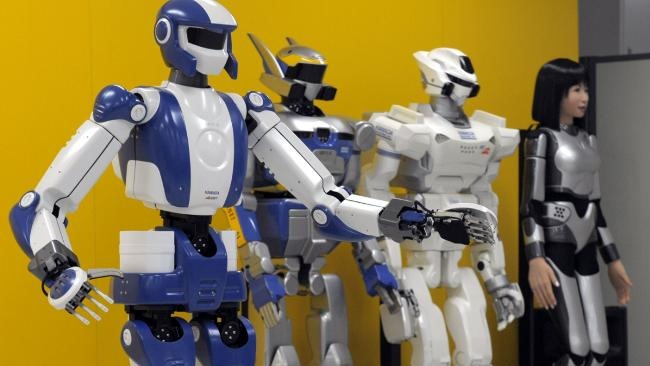
\includegraphics[width=\linewidth]{src/chap0-introduction/hrp_family.jpg}
  \end{center}
  \caption{Les robots HRP-4, HRP-2, HRP-3 et HRP-4c (de gauche à
    droite). \label{fig:hrpfamily}}
\end{figure}

Les robots humanoïdes se divisent en deux catégories: ceux de petite
taille comme le robot Nao d'Aldebaran Robotics \citep{wikipedia.nao}
et les humanoïdes de grande taille tels que ceux développés dans le
cadre du projet HRP ou bien encore par les sociétés avec le robot
Partner ou Honda avec robot Asimo. Les problématiques posées par les
deux types d'humanoïde sont assez différentes. Les robots de petite
taille utilisent des actionneurs moins puissants, de qualité moindre,
sont d'une conception moins précise par ils utilisent souvent des
squelettes en plastique plutôt qu'en métal pour des questions de
coût. Leurs capacités de calcul sont également souvent très limitées
au point qu'un ordinateur externe est souvent nécessaire pour les
commander. Les enjeux sont donc ici comment limiter les calculs
nécessaires à bord du robot étant donné les fortes contraintes sur la
capacité de calcul, comment prendre en considération les imperfections
dans la modélisation du robot, la flexibilité de ses différentes
parties ou bien encore la mauvaise précision de ses
actionneurs. L'objectif étant de fournir à moyen terme un robot
compagnon réalisant des tâches simples comme jouer avec un humain ou
fournir des services simples comme la télésurveillance. Les capacités
de manipulation de ces humanoïdes sont, à l'heure actuelle, très
limitées, voire inexisantes.


Au contraire, les grands humanoïdes sont extrêmement onéreux et
composés de pièces usinées très précisément et d'actionneurs
extrêmement performants. De ce fait, les problèmes d'identification de
modèles ne se posent qu'à la marge et le mouvement réel du robot est
très proche de sa simulation faisant l'hypothèse de mouvements de
corps rigides. Les capacités de calcul sont également plus importantes
bien qu'inférieures à ce que l'on peut trouver dans un robot mobile où
un poids important ne pose pas de problème particulier. Selon les
modèles, ces robots peuvent réaliser des tâches de manipulation
complexe. Les défis posés par ces robots sont différents: ils sont
plus lourds, plus grands et donc toute chute leur est généralement
fatale. La commande à gain fort courante sur ce type de système rend
également le comportement du système potentiellement dangereux: pour
atteindre sa consigne, le robot aura tendance à appliquer le couple
maximal de ses actionneurs, quitte à s'endommager lui-même ou à
blesser un humain se trouvant à proximité. Ils restent donc, à l'heure
actuelle, des outils de recherches dangereux impropres à une
utilisation à proximité d'humains.


\subsection{Le projet japonais HRP}


\begin{figure}
  \begin{center}
    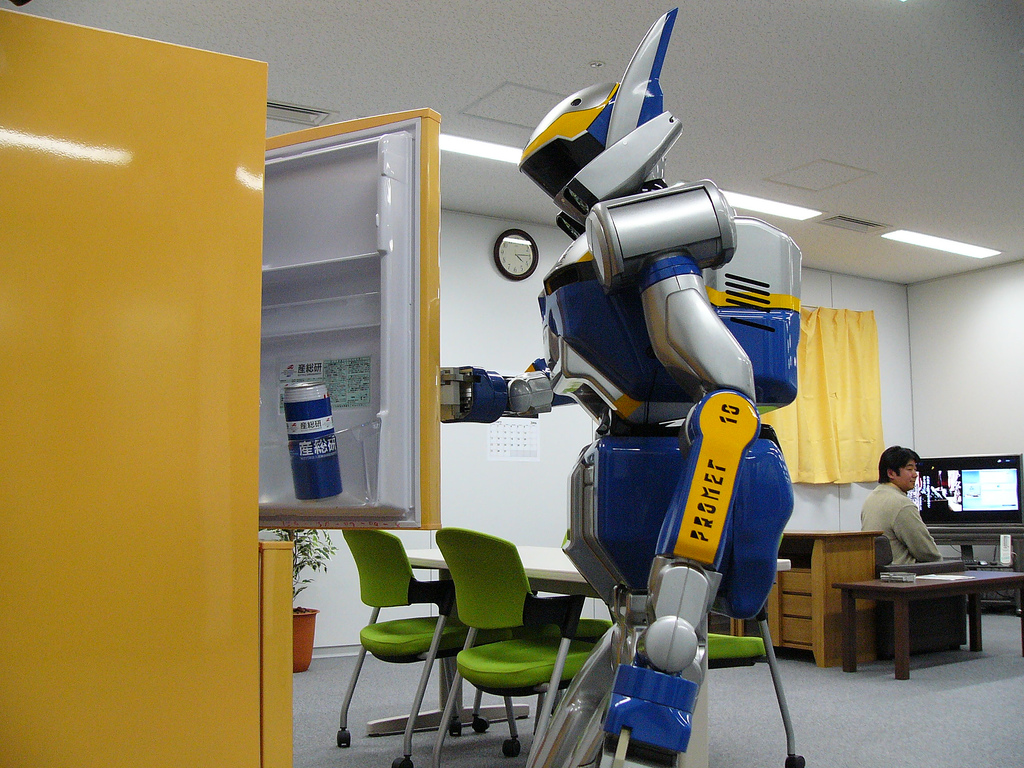
\includegraphics[width=\linewidth]{src/chap0-introduction/hrp2.jpg}
  \end{center}
  \caption{Le robot HRP-2\index{HRP-2} réalisant une tâche de
    manipulation. \label{fig:hrp2}}
\end{figure}


La totalité des recherches effectuées durant cette thèse et qui sont
décrites ici ont été validées sur la plate-forme robotique HRP-2
\citep{04kaneko.icra} du LAAS. Une version alternative est illustré
par la \autoref{fig:hrp2}. Le robot humanoïde HRP-2 ``Promet'' est un
robot humanoïde japonais mesurant 154cm et pesant 58kg. Il dispose de
deux jambes à six degrés de liberté, de deux bras à six degrés et de
deux mains à un degré de liberté commandant l'ouverture de la pince
composant chaque préhenseur. Deux degrés de liberté sont affectés au
mouvement de la tête et les deux derniers actionnent l'articulation du
torse du robot. Cette dernière étant une caractéristique unique de
cette plate-forme. Le nombre total de degrés de liberté du système est
donc de 30. Les capteurs de ce robot comprennent quatre capteurs de
force six-axes aux chevilles et au poignet, ainsi qu'une centrale
inertielle dans le torse mesurant la vitesse angulaire et
l'accélération linéaire du torse. Un système de caméras composé de
deux paires stéréo situées dans la tête est également présent. Une
première paire possède des objectifs grand-angles permettant de
percevoir une large portion de l'environnement entourant le robot
tandis que la seconde a un angle de vue plus étroit, permettant une
bonne précision lors de la manipulation. Ce robot dispose d'un système
absorbant les chocs dans chaque cheville afin de protéger la mécanique
des impacts réalisés pendant la marche. Les traitements embarqués sont
réalisés par deux ordinateurs reliés entre eux par un réseau
Ethernet. La connexion avec l'extérieur est assurée par un point
d'accès WiFi.


Ce robot conçu en 1998 a été suivi du robot HRP-3 en 2007, du robot
HRP-4C en 2009 et du robot HRP-4 en 2010. HRP-3 s'est démarqué en
étant le premier robot humanoïde résistant à l'eau ouvrant la porte à
une utilisation de ces robots en extérieur. HRP-4c est un gynoïde,
c'est-à-dire un robot humanoïde possédant l'apparence d'une femme. Les
applications ciblent le domaine du mannequinat et du divertissement
plus généralement. Le dernier robot de la série, HRP-4 est, quant à
lui, plus léger tout en conservant sept degrés de liberté pour les
bras et deux degrés de liberté pour les mains. Les différents modèles
sont illustrés par la \autoref{fig:hrpfamily}.


\section[Contributions]{Contributions, de la génération de mouvements à leur exécution}


Le maître mot de ces trois ans et demi est finalement, et cela ne peut
que se ressentir à la lecture de ce manuscrit, la polyvalence. Comme
dans toute thèse expérimentale, il a été nécessaire de tenter de
mettre en pratique des idées, de A à Z. C'est à la fois formateur et
passionnant, mais m'a conduit à utiliser de très nombreux outils,
algorithmes de l'État de l'Art et à les comprendre afin de pouvoir les
intégrer à l'approche que j'ai souhaité développer. Le travail réalisé
étant principalement de faire communiquer les idées entre elles:
comment un algorithme de vision peut-il servir la commande? Comment
les données capteur peuvent-elles être utilisées par différents
composants?  Autant de questions qui, en terme d'ingénierie
logicielle, consistent à lier des boîtes entre elles, encapsulant
autant d'algorithmes et de stratégies de décision différentes. Il est
toutefois difficile d'argumenter sur la pertinence des ``flèches''
sans expliquer au préalable ce que contiennent les ``boîtes'',
d'autant que si certaines techniques sont classiques en robotique,
d'autres sont issues des recherches du groupe GEPETTO et ne peuvent
être considérées comme allant de soi. Le choix réalisé lors de la
rédaction a donc été d'expliquer progressivement comment réaliser des
scénarii complexes avec un robot humanoïde, de la théorie, à la
pratique, mes contributions se situant davantage dans ce spectre. Le
premier chapitre de ce manuscrit traite d'un problème particulier
abordé dans le cadre de cette thèse: la représentation informatique
des problèmes d'optimisation numérique. Ce problème peut sembler
distinct de la robotique humanoïde, mais les techniques d'optimisation
sont devenues un socle supportant tant d'algorithmes utiles qu'on ne
peut pas éluder la question de la représentation de ces
problèmes. L'objectif ici est de s'appuyer sur les caractéristiques
des langages de programmation modernes, tel que le C++ afin de pouvoir
définir un problème d'optimisation une fois puis de pouvoir le
transmettre à différents solveurs de façon transparente. Une
application robotique simple valide cette approche, mais la
contribution majeure reste la formulation et la modélisation
informatique du problème. Le second chapitre explique pas à pas les
techniques de génération de mouvement et d'exécution sur le robot. Ces
techniques font partie de l'État de l'Art et il n'y a pas d'apport
original à ce niveau. Cependant, le contrôleur construit sur ces
techniques et permettant de suivre des trajectoires tout en
incorporant les données capteur est un travail totalement original et
sur lequel, à notre connaissance, aucun article antérieur n'a été
publié. Le troisième chapitre est divisé en deux: tout d'abord la
description informatique d'une pile de tâches asservie est un apport
original. La suite du chapitre est dédiée à la localisation utilisant
la vision sur un robot humanoïde. Cette partie n'est pas nouvelle en
soi, car des résultats similaires ont déjà été publiés dans ce
domaine, mais l'intégration de la localisation au schéma de contrôle
proposé dans le \autoref{chap:suivi} est un travail original. Le
dernier chapitre traite de l'intégration des différents composants sur
notre plate-forme robotique. Dans ce chapitre, la totalité des
algorithmes proposés font, soit partie de l'État de l'Art, soit ont été
conçus par d'autres équipes partenaires du LAAS, notamment l'équipe
\mbox{LAGADIC} de l'IRISA à Rennes. L'apport original de cette partie
consiste à démontrer comment on peut construire une architecture
robotique complète en utilisant des algorithmes existant afin
d'atteindre des comportements de plus haut niveau.

\chapter{Path Optimization for Humanoid Walk Planning: an Efficient Approach}
\label{chap:path-optim}

This chapter deals with path optimization for humanoid walk planning
in cluttered environments. Under the assumption that the humanoid
robot will walk on a flat floor in a perfectly modeled static
environment, it presents a heuristic and efficient optimization method
that takes as input a path computed for the humanoid bounding box, and
produces a path where a discrete set of configurations is reoriented
using an A$^{*}$ search algorithm. A pattern generator is then used to
generate a trajectory that is realistic and time-optimal. This method
is validated in various scenarios on the humanoid robot HRP-2.

\section{Motion Planning in the Configuration Space}
\label{sec:chap1-motion-planning}

The problem of motion planning is now well formalized in robotics and
several books present the various approaches
\cite{lato91,chos05,lava06}. One particularly useful concept is the
one of configuration space (denoted by \cspace) \cite{loza83}, which
is the set of all configurations \config{} of a robot \robot;
\config{} is a vector comprised of the $n$ independent degrees of
freedom (DoF) that are sufficient to know the full state of the robot
at each instant. \cspace defines then a submanifold of \espace. Some
of the robot body positions can generate (self-)collisions; the
equivalent configurations will be said to be in collision, and the set
of all configurations in collision is denoted by \cobs
$\subset$ \cspace. Its complementary is denoted by \cfree and is
called the free configuration space. Using these notations, we can
redefine the motion planning problem as the answer to the following
question: is there a continuous path $P: [0,1] \rightarrow$ \cfree
that connects a start configuration \config{s} to a goal configuration
\config{g}, and what is it?

\subsection{Deterministic Algorithms}
\label{subsec:chap1-deterministic algorithms}

This question can be answered through the use of deterministic
algorithms; for a given number of tries, they will always compute the
same valid path $P$.

FIXME: not precise
One class of algorithms, mainly developed in the past 30 years, relies
on representing \cobs explicitly in order to build a graph, also
called roadmap, that represents the connectivity of \cfree. Solving
the motion planning problem then boils down to a graph exploration to
connect \config{s} to \config{g}. A non-exhaustive list of these
methods includes cellular decomposition, Voronoi diagrams, visibility
graphs, and Canny's algorithm \cite{good04}.

Such algorithms offer the nice property of completeness, i.e. they can
always give a full answer to the motion planning problem as defined
previously. But while they work well for solving path planning
problems in low-dimensional configuration spaces, their computational
cost becomes penalizing in high-dimensional configuration spaces. In
fact building \cfree requires finding its frontiers, and computation
time is at best exponential with respect to the dimension of \cspace.

Other approaches are inspired from real-time motion generation
techniques, such as the one detailed in \cite{khat85}, which consists
in assigning artificial attractive potentials on the goals, and
repulsive ones around the start configuration and the obstacles. The
robot is then subject to forces that will direct it from the start
configuration towards the goal configuration. However, because of the
locality of the planner, a path may be computed while not being a
solution to the path planning problem. This can happen in a maze-like
environment when a stable equilibrium point other than the goal
configuration is found (see Figure
\ref{fig:chap1-deterministic-algorithm}).

\begin{figure}
  \centering
      {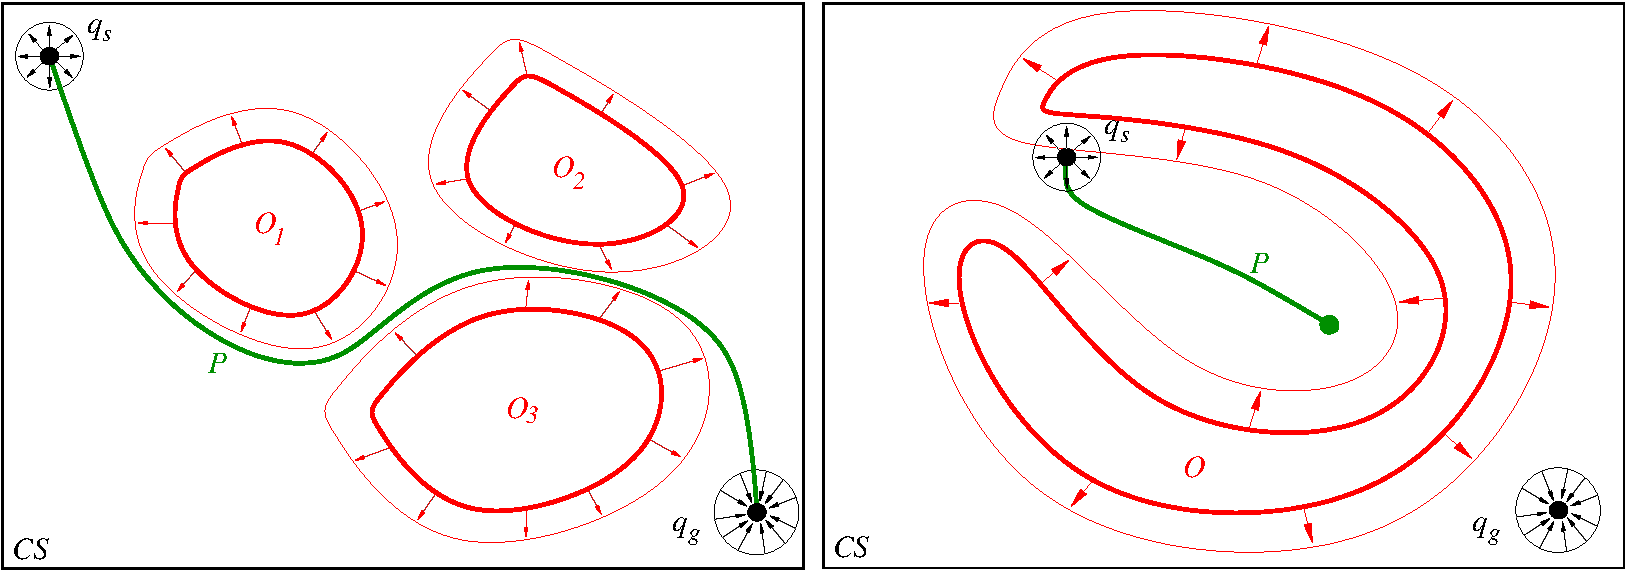
\includegraphics[width = \linewidth]
        {src/chap1-path-optimization/deterministic-algorithm.pdf}}
      \caption{Left: A valid path is computed by the deterministic
        algorithm. Arrows show the attractive and repulsive potential
        fields. Thin lines show the potential lines. Right: Example of
        problem where the stable local minimum does not coincide with
        the goal configuration. $P$ is thus not a solution to the path
        planning problem.}
      \label{fig:chap1-deterministic-algorithm}
\end{figure}

\subsection{Sampling-based Algorithms}
\label{subsec:chap1-sampling-algorithms}

Deterministic algorithms rapidly reach their limit when the
configuration space dimension rises above 4. Computation speed plays a
big part in choosing which algorithm to use for path planning
problems, as many applications require, or at least aim for, real-time
resolution. In this perspective, sampling-based algorithms, such as
Probabilistic Roadmaps (PRM) \cite{kavr96} or Rapidly-exploring Random
Trees (RRT) \cite{kuff00}, were developed in the past fifteen years.

Instead of trying to build an explicit representation of \cfree,
sampling-based algorithms rely on approximating the connectivity of
\cfree through rejection sampling: random configurations \config{rand}
are sampled in \cspace, and efficient Boolean collision detection
techniques \cite{huds97, gott96} reject configurations that produce
collisions, keeping only configurations \config{} $\in$ \cfree.

The classic RRT algorithm, as presented in \cite{kuff00}, relies on
the Voronoi bias to efficiently explore \cfree and grow a random tree
in it. Each iteration of the algorithm attempts to extend the tree by
adding new vertices in the direction of a randomly selected
configuration \config{rand}. Algorithm~\ref{alg:chap1-rrt} shows the
pseudo-code of the RRT algorithm. It takes as input an initial
configuration \config{s} and grows a tree \ctree rooted in \config{s}.

\begin{algorithm}
\caption{RRT(\config{s})}
\label{alg:chap1-rrt}
\begin{algorithmic}
\STATE \ctree$.$Init$($\config{s}$)$
\FOR{$i$ = 1 to $K$}
\STATE \config{rand} $ \leftarrow $ Rand$($\cspace$)$
\STATE \config{near}$ \leftarrow $ Nearest$($\config{rand}$,$\ctree$)$
\STATE Extend$($\ctree$,$\config{near}$,$\config{rand}$)$
\ENDFOR
\end{algorithmic}
\end{algorithm}

One way to make the RRT algorithm more efficient is to grow trees from
both the initial and goal configurations, see Figure
\ref{fig:chap1-rrt}. This was first proposed in \cite{kuff00}.

\begin{figure}
  \centering
      {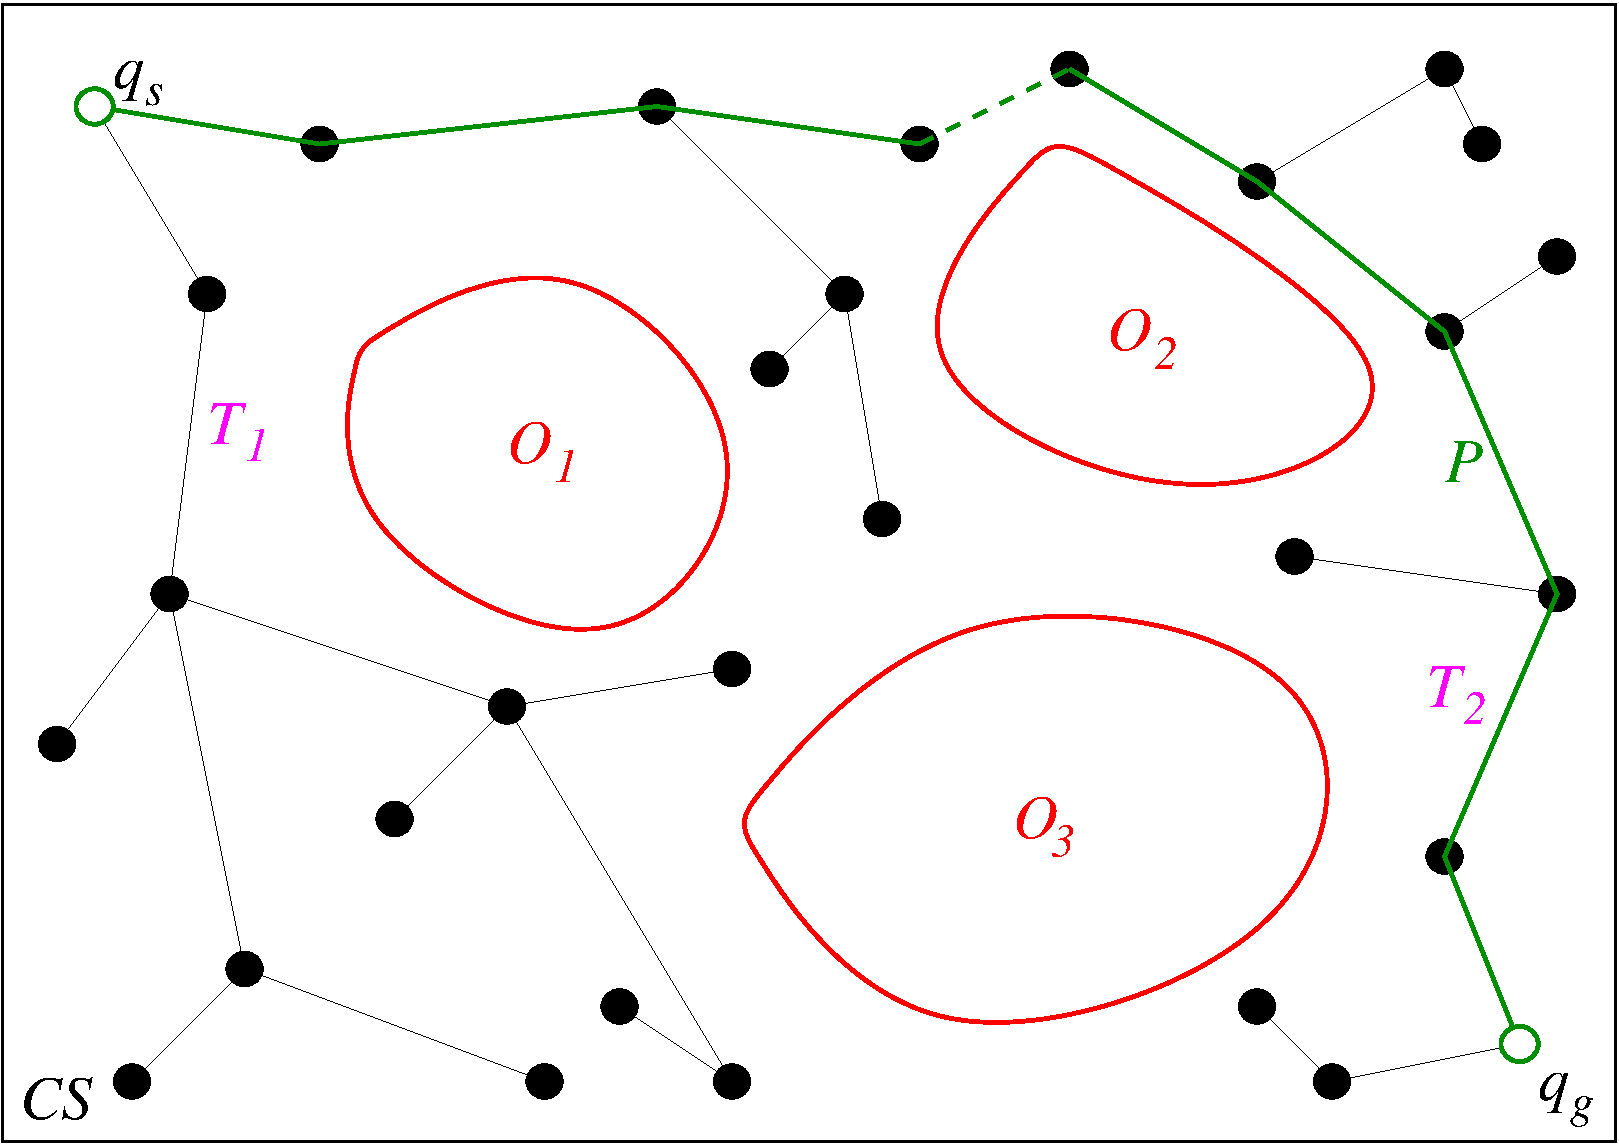
\includegraphics[width = 0.8\linewidth]
        {src/chap1-path-optimization/rrt.pdf}}
      \caption{A valid path (in green) computed with a bidirectional
        RRT planner. $q_{start}$ and $q_{goal}$ are the roots of the
        trees $\mathcal{T}_{1}$and $\mathcal{T}_{2}$ respectively. The
        algorithm keeps diffusing both trees until they can be
        connected together with an edge (in dashed green).}
      \label{fig:chap1-rrt}
\end{figure}

While not being resolution complete (i.e. they cannot tell whether a
solution exists or not), sampling-based algorithms have the less
strong property of probabilistic completeness: if a solution path
exists, the algorithm will be able to compute it with a probability of
$1$ when the number of iterations $K$ reaches infinity. This may seem
like a very weak property, but in practice these algorithms can
compute paths in complex real-life environments in a reasonable time
on regular computers and have been used to solve problems for various
systems, ranging from 6-DoF floating objects, 50-DoF anthropomorphic
systems, to 1000-DoF proteins.

\subsection{Path Optimization}
\label{subsec:chap1-path-optimization}

As shown in Figure \ref{fig:chap1-rrt}, RRT returns the shortest path
$P$ inside the graph that connects \config{s} to \config{g}. Due to
the probabilistic nature of RRT, it is clear that $P$ is not optimal
in terms of length. Path optimization methods take a valid,
i.e. collision-free, path as input and try to shorten while making
sure that the output path is still valid.

\subsubsection{Greedy Optimization}

A greedy optimizer, such as the one shown in Figure
\ref{fig:chap1-optimizers}, uses the greedy approach to shorten and
smooth a path. First, it tries to connect directly \config{s} to
\config{g}; if the path is collision-free, it tries to connect
\config{s} to the node preceding \config{g}, and so on until it
reaches \config{s}. This process is then restarted similarly on the
following nodes.

\subsubsection{Random Optimization}
\label{subsubsec:chap3-random-optimization}

In the case of the greedy optimizer, the nodes that are in the
optimized path are also nodes of the input path. Random Optimization
(RO) tries to bypass some nodes and keeps the rest. While this simple
method runs very fast, it does not always give the best possible
path. A different shortcut strategy can be run in a loop: at each
iteration, two random configurations are sampled on the path, and the
optimizer tries to connect \config{s} to the first, the first one to
the second one, and the second one to \config{g}. The local paths that
are still collision-free are then kept to make a shorter path, as
shown in Figure \ref{fig:chap1-optimizers}.

\begin{figure}
  \centering
      {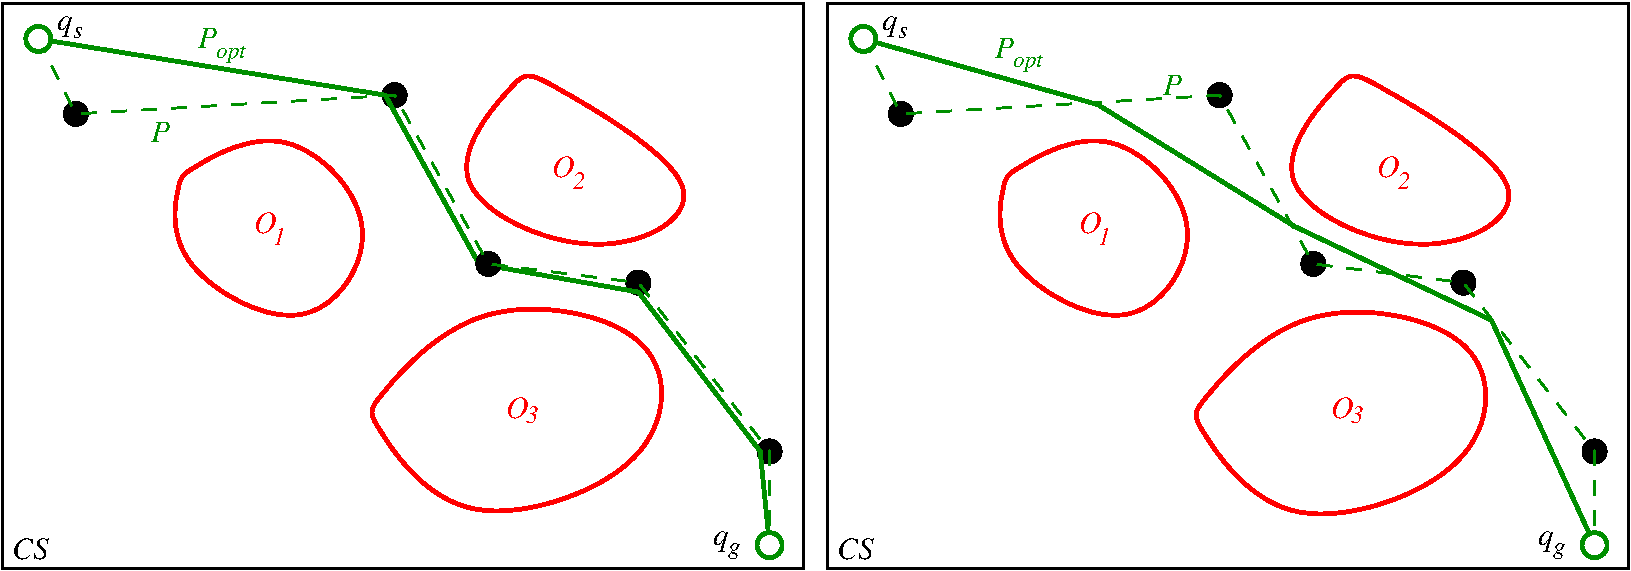
\includegraphics[width = \linewidth]
        {src/chap1-path-optimization/optimizers.pdf}}
      \caption{Left: The path $P$ (in dashed green) is optimized with
        a greedy optimizer. Right: The optimized path $P_{opt}$ (in
        continuous green) after several iterations of random
        optimization (RO).}
      \label{fig:chap1-optimizers}
\end{figure}

\section{Anthropomorphic Systems}
\label{sec:chap1-anthropomorphic-systems}

We focus in this work on humanoid robots and digital actors, which are
anthropomorphic systems. Such systems have a high number of DoF, and
are capable of accomplishing human-like tasks: locomotion(such as
walking, running and parkour), manipulation, or both. These tasks can
be accomplished thanks to the fact that anthropomorphic systems are
both underactuated and highly-redundant.

In the remainder of this work, we will refer indistinguishably to
anthropomorphic systems, humanoid robots and digital actors.

\subsection{Underactuated Systems}
\label{subsec:chap1-underactuated-systems}

A robot \robot usually composed of a set of rigid bodies \body{i}, $i
\in 0..N_B$, and a set of joints \joint{i}, $i \in 1..N_J$, which
constrain the body positions. A rigid body has a mass, an inertia, and
a given geometry. We use the kinematic tree formalism proposed in
\cite{feat08} to model a full robot: a node of the tree represents a
body of the robot, while an arc (or edge) represents a joint \joint{i}
of the robot which constrains the motion of the successor body
\body{i} with respect to its parent body \body{\lambda_{i}} (see
Figure \ref{fig:chap1-robot-kinematic-tree}). Note that in the tree
representation, each body has one and exactly one parent body, except
for the root body which has no parents; this means that additional
constraints have to be added later on in order to correctly model
robots with closed kinematic chains such as parallel robots.

\begin{figure}
  \centering
      {\def\svgwidth{0.8\linewidth}
        \subimport*{src/chap1-path-optimization/}
                   {robot-kinematic-tree.pdf_tex}}
      \caption{Left: schematic view of a humanoid robot: bodies
        are connected with joints (yellow circles) which represent the
        actuators. A fictitious 6-DoF joint, or floating joint (purple
        circle), is added to move the robot in \segroup. Right: A
        kinematic tree view of the same robot, where bodies and joints
        are represented by nodes and joints respectively.}
      \label{fig:chap1-robot-kinematic-tree}
\end{figure}

Joints usually correspond to the actuators on the physical robot. Each
type of actuator will then have an equivalent type of joint
(prismatic, revolute, etc). A configuration \config{} of such a robot
can then be defined as the concatenation of all joint DoF values, and
the set of all configurations is called the actuated configuration
space \actcspace. This is however not sufficient in the particular
case of anthropomorphic systems, which rely on making and breaking
contact with their environment -- the floor for instance -- in order
to move in their workspace. Additional information in the
configuration vector is needed to model the general position of the
system, and not only its actuators. Anthropomorphic systems are
therefore said to be unactuated systems.

We therefore introduce a 6-DoF floating joint, which we attach to the
root of the existing kinematic tree containing the actuated
joints. The successor body of the floating joint will be called the
floating base. Note that any body of the kinematic tree can be chosen
to be the floating base; in Figure
\ref{fig:chap1-robot-kinematic-tree}, the floating base is the
``waist'' of the robot. Thus, a full configuration \config{} of the
robot \robot is an element of the configuration space \cspace $=$
\segroup $\times$ \actcspace.
 
\subsection{Kinematic Redundancy}
\label{subsec:chap1-kinematic-redundancy}

\begin{figure}
  \centering
      {\def\svgwidth{0.8\linewidth}
        \subimport*{src/chap1-path-optimization/}
                   {robot-redundancy.pdf_tex}}
      \caption{Anthropomorphic systems are highly-redundant
        systems. For a desired Cartesian position (in blue) of the end
        effector \body{e}, there exists more than one configuration
        \config{} that accomplishes this task. Left and right: two
        possible solution configurations.}
      \label{fig:chap1-robot-redundancy}
\end{figure}

We briefly introduce here the concept of kinematic redundancy. Figure
\ref{fig:chap1-robot-redundancy} shows that for a same target
Cartesian position of the end effector \body{e}, there exists more
than one configuration of \robot that allows \body{e} to reach the
target. The robot \robot is therefore kinematically redundant with
respect to the task of reaching the object. One could imagine
assigning multiple tasks to be accomplished at the same time, or even
exploring \cspace while continuously accomplishing one or more
tasks. This will be discussed in more thoroughly in Chapter
\ref{chap:wholebody-planning}.

\section{Walk Pattern Generation}
\label{sec:chap1-pattern-generator}

An important field of humanoid robotics research is the generation of
dynamically balanced walk patterns. Since the introduction of the
Zero-Moment Point (ZMP) \cite{vukobratovic1969contribution}, several
methods have been proposed to generate walking motions efficiently.

\subsection{Zero-Moment Point (ZMP)}
\label{subsec:chap1-zmp}

We assume here that the robot \robot is walking on a flat horizontal
floor. We also assume that the robot is always making contact with the
floor, i.e. that there are no jumps, and that all contacts are
non-sliding. \robot is then subject to its weight and to contact
forces.

Under these assumptions, \cite{vukobratovic1969contribution} define
the Zero-Moment Point (ZMP) as the point on the floor where the
horizontal components of the sum of moments applied to \robot are
zero. It is also established that \robot will not tilt around its foot
edges as long as the ZMP lies inside the support polygon, i.e. the
convex hull of all contact points, which are coplanar due to the
previous assumptions. This is known as the condition of dynamic
balance, and the robot \robot is then said to be dynamically
balanced. We will discuss more the complete ZMP formulation in Chapter
\ref{chap:optimal-motion-planning}.

Note that in the particular case where speed and acceleration are
zero, the ZMP will coincide with the CoM vertical projection on the
floor; the robot \robot will then be said to be statically balanced if
this projection lies inside the support polygon.

\subsection{Cart-Table Model}
\label{subsec:chap1-cart-table}

The above formulation of ZMP is rather hard to control.  One way to
deal with the complexity of a humanoid robot kinematic tree is to use
the so-called "cart-table" simplified model, where the walking robot
is modeled by a point mass at a fixed height.  The equations giving
the ZMP horizontal coordinates $(p_x,p_y)$ as functions of the center
of mass (CoM) horizontal coordinates $(x,y)$ in the cart-table model
were presented in \cite{kaji03}:
\begin{equation}
\label{eq:chap1-walk-zmp}
\left(
\begin{array}{c}
p_x\\ p_y
\end{array}
\right) = \displaystyle \left(
\begin{array}{c}
x - \frac{z_c}{g} \ddot{x}\\ y - \frac{z_c}{g} \ddot{y}
\end{array}
\right)
\end{equation}
where $z_c$ is the constant height of the CoM and $g$ is the gravity
constant.

\begin{figure}
  \centering
      {\def\svgwidth{0.5\linewidth}
        \subimport*{src/chap1-path-optimization/}
                   {robot-cart-table.pdf_tex}}
      \caption{Simplified model of a cart on table. The cart can move
        horizontally along one dimension on the table with a non-zero
        acceleration and represents the robot CoM. The table foot
        represents the contact surface of the robot. Note that in its
        current state, the robot is dynamically balanced, as the ZMP
        lies on the table foot. The CoM vertical projection, on the
        other hand, doe not, and static balance is not ensured.}
      \label{fig:chap1-robot-cart-table}
\end{figure}

Based on this model, planning a trajectory for the ZMP is reduced to
planning a trajectory for CoM of the robot. Given a trajectory of the
CoM and footprint positions, inverse kinematics solvers can animate
the whole set of DoF of the robot to generate a dynamically balanced
walk trajectory.

\begin{figure}
  \centering
  \definecolor{c8eff88}{RGB}{142,255,136}
\definecolor{cffc925}{RGB}{255,201,37}
\definecolor{cff5663}{RGB}{255,86,99}
\definecolor{c454545}{RGB}{69,69,69}
\definecolor{c0200d1}{RGB}{2,0,209}

\begin{tikzpicture}[y=2.pt, x=2.pt,yscale=-1, inner sep=0pt, outer sep=0pt]
  %Start and end configurations
  \begin{scope}[cm={{0.0,1.0,-1.0,0.0,(360.33128,174.24827)}}]
    \path[draw=black,fill=c8eff88,miter limit=4.00,line width=0.800pt,rounded
      corners=0.0000cm] (47.0740,258.0597) rectangle (81.6792,276.2132);
    \path[draw=black,fill=c8eff88,line join=miter,line cap=butt,line width=0.800pt]
    (64.1273,257.7760) -- (64.1273,246.9973);
    \path[draw=black,fill=c8eff88,line join=miter,line cap=butt,line width=0.800pt]
    (64.1273,246.4300) -- (67.6730,250.2593) -- (60.8654,250.2593) -- cycle;
  \end{scope}
  \begin{scope}[cm={{0.0,1.0,-1.0,0.0,(478.33128,174.24827)}}]
    \path[draw=black,fill=c8eff88,miter limit=4.00,line width=0.800pt,rounded
      corners=0.0000cm] (47.0740,258.0597) rectangle (81.6792,276.2132);
    \path[draw=black,fill=c8eff88,line join=miter,line cap=butt,line width=0.800pt]
    (64.1273,257.7760) -- (64.1273,246.9973);
    \path[draw=black,fill=c8eff88,line join=miter,line cap=butt,line width=0.800pt]
    (64.1273,246.4300) -- (67.6730,250.2593) -- (60.8654,250.2593) -- cycle;
  \end{scope}
  %Footprints
    \path[cm={{0.0,1.0,-1.0,0.0,(0.0,0.0)}},draw=black,fill=cffc925,miter
      limit=4.00,line width=0.800pt,rounded corners=0.0000cm] (225.3161,-100.2912)
    rectangle (235.2439,-86.1087);
    \path[cm={{0.0,1.0,-1.0,0.0,(0.0,0.0)}},draw=black,fill=cffc925,miter
      limit=4.00,line width=0.800pt,rounded corners=0.0000cm] (225.3161,-144.2911)
    rectangle (235.2439,-130.1087);
    \path[cm={{0.0,1.0,-1.0,0.0,(0.0,0.0)}},draw=black,fill=cffc925,miter
      limit=4.00,line width=0.800pt,rounded corners=0.0000cm] (225.3161,-174.2911)
    rectangle (235.2439,-160.1087);
    \path[cm={{0.0,1.0,-1.0,0.0,(0.0,0.0)}},draw=black,fill=cffc925,miter
      limit=4.00,line width=0.800pt,rounded corners=0.0000cm] (225.3161,-202.2911)
    rectangle (235.2439,-188.1087);
    \path[cm={{0.0,1.0,-1.0,0.0,(0.0,0.0)}},draw=black,fill=cffc925,miter
      limit=4.00,line width=0.800pt,rounded corners=0.0000cm] (225.3161,-218.2911)
    rectangle (235.2439,-204.1087);
    \path[cm={{0.0,1.0,-1.0,0.0,(0.0,0.0)}},draw=black,fill=cff5663,miter
      limit=4.00,line width=0.800pt,rounded corners=0.0000cm] (242.4480,-100.2912)
    rectangle (252.3757,-86.1087);
    \path[cm={{0.0,1.0,-1.0,0.0,(0.0,0.0)}},draw=black,fill=cff5663,miter
      limit=4.00,line width=0.800pt,rounded corners=0.0000cm] (242.6932,-130.9444)
    rectangle (252.6209,-116.7619);
    \path[cm={{0.0,1.0,-1.0,0.0,(0.0,0.0)}},draw=black,fill=cff5663,miter
      limit=4.00,line width=0.800pt,rounded corners=0.0000cm] (242.6932,-158.9444)
    rectangle (252.6209,-144.7619);
    \path[cm={{0.0,1.0,-1.0,0.0,(0.0,0.0)}},draw=black,fill=cff5663,miter
      limit=4.00,line width=0.800pt,rounded corners=0.0000cm] (242.6932,-186.9444)
    rectangle (252.6209,-172.7619);
    \path[cm={{0.0,1.0,-1.0,0.0,(0.0,0.0)}},draw=black,fill=cff5663,miter
      limit=4.00,line width=0.800pt,rounded corners=0.0000cm] (242.8937,-218.4225)
    rectangle (252.8214,-204.2401);
  %ZMP trajectory
    \path[draw=c454545,line join=miter,line cap=butt,miter limit=4.00,line
      width=0.800pt] (92.6635,239.1801) -- (92.6635,229.8536) -- (124.1530,247.9049)
    -- (137.5913,229.8536) -- (152.2329,247.9049) -- (167.2757,230.0542) --
    (180.3127,247.3032) -- (195.5561,230.2548) -- (211.8023,247.9049) --
    (211.8023,238.6787);
  %Com trajectory
    \path[draw=c0200d1,line join=miter,line cap=butt,miter limit=4.00,line
      width=0.800pt] (92.5632,239.1801) .. controls (92.3626,227.5470) and
    (108.6088,239.0798) .. (108.6088,239.0798) .. controls (123.1502,247.7044) and
    (130.9724,238.6787) .. (130.9724,238.6787) .. controls (137.3907,229.5528) and
    (145.3132,239.2804) .. (145.3132,239.2804) .. controls (152.2329,247.5038) and
    (159.7543,239.0798) .. (159.7543,239.0798) .. controls (167.4762,229.0513) and
    (173.9948,239.1801) .. (173.9948,239.1801) .. controls (180.3127,247.5038) and
    (187.6336,238.8793) .. (187.6336,238.8793) -- (187.7338,238.6787) .. controls
    (196.9601,227.8479) and (203.3783,238.7790) .. (203.3783,238.7790) .. controls
    (211.9026,248.3061) and (211.8023,238.6787) .. (211.8023,238.6787);
  %legend
    \path[opacity=0,line join=miter,line cap=butt,line width=0.800pt]
    (85,200.7535) -- (100,200.7535)
    node[opacity=0,right] {\footnotesize Desired ZMP trajectory};
    \path[draw=c454545,line join=miter,line cap=butt,line width=0.800pt]
    (85,200.7535) -- (100,200.7535)
    node[right=2] {\footnotesize Desired ZMP trajectory};
    \path[draw=c0200d1,line join=miter,line cap=butt,line width=0.800pt]
    (85,206) -- (100,206)
    node[right=2] {\footnotesize CoM trajectory};

\end{tikzpicture}

  \caption{An illustration of the walking pattern generator: a desired
    ZMP trajectory (in grey) connects footprints. During the
    single-support phase, the ZMP stays under the support foot, and
    switches feet during the double support phase. The cart-table
    model is then used to produce the corresponding CoM trajectory (in
    blue).}
  \label{fig:chap1-zmp}
\end{figure}

\section{Humanoid Walk Planning}
\label{sec:chap1-humanoid-walk-planning}

The motion planning problem is certainly a complex one in the case of
humanoid robots, which are high-DoF redundant systems that have to
verify bipedal stability constraints. Various planning strategies can
be found in literature.

\subsection{Footstep Planning}
\label{subsec:chap1-footstep-planning}

One possible way of addressing humanoid walk planning is by reasoning
on the footstep level. Works of \cite{kuff01,ches05} describe humanoid
footstep planning schemes. Starting from an initial footstep
placement, they use an A$^{*}$ graph search \cite{hart68} to explore a
discrete set of footstep transitions. The search stops when the
neighborhood of the goal footstep placement is reached. This approach
is not practical in some environments with narrow passages, and
\cite{xia09, perr11a} reduced the computational cost of footstep
planning by adapting RRT planning algorithm and efficiently exploring
the discrete footstep space. In their most recent work, \cite{perr11b,
  perr12} give an elegant proof of the equivalence between discrete
footstep planning and a continuous motion planning, which enables the
use of off-the-shelf planning algorithms such as RRT.

\subsection{Constraints-Based Motion Generation}
\label{subsec:chap1-constraints-motion-generation}

Another category relies on prioritized whole-body task planning:
kinematic redundancy is used to accomplish tasks with different orders
of priorities \cite{khat04, saab-tro-12}. Dynamic balance and obstacle
avoidance can then be defined as unilateral constraints that the
algorithm has to verify during the whole motion. The trajectory is
then generated by specifying a set of goal tasks -- which could be a
goal configuration -- and let this set act as an attractor, in a way
similar to the simpler example shown in
\ref{subsec:chap1-deterministic algorithms}. Using such as scheme,
\cite{kano09} defines a robot augmented with a sequence of footprints
and formulates the problem of locomotion planning as an optimization
problem. Such as scheme works well in the presence of simple
obstacles, but is prone to falling and local minima failing to find
solutions in more complex environments.

\subsection{Constrained Motion Planning}
\label{subsec:chap1-constrained-motion-planning}

More recently, sampling-based motion planning algorithms were adapted
to efficiently explore a constraint submanifold of \cspace. In
\cite{bret06, haus10}, this strategy is used to plan on a union of
submanifolds, where each manifold is defined by a contact limb
position and static balance constraints, producing statically balanced
locomotions for hexapods and humanoid robots on uneven
terrain. Constrained motion planning will be further discussed in
Chapter \ref{chap:wholebody-planning}, where a new dynamically-balanced locomotion
planner is introduced.

\subsection{Multi-Contact Planning}
\label{subsec-chap1-multi-contact-planning}

It is interesting to note that while collision avoidance is a
requirement in motion planning, some features of the environment can
in fact be useful to solve the problem, especially in the case of
underactuated systems. \cite{esca06, bouy12} propose a
multiple-contact-point stance planner that looks for authorized
contacts in order to help the robot reach its goal.

\subsection{Decoupled Planning}
\label{subsec:chap1-bounding-box}

Finally, Another strategy consists of dividing a high-dimensional
problem into smaller problems and solving them successively
\cite{zhan09}. The idea of dividing the problem into a two-stage
scheme is described in \cite{yosh08}: A 36-DoF humanoid robot is
reduced to a 3-DoF bounding box. Using the robot simplified model, the
PRM algorithm solves the path planning problem and generates a valid
path for the bounding box. A geometric decomposition of the path
places footsteps on it, and the walk pattern generator described in
\ref{sec:chap1-pattern-generator} finally produces the whole-body
trajectory for the robot. In \cite{moul10}, this two-stage approach is
also used; numerical optimization of the bounding box path produces a
time-optimal trajectory that is constrained by foot speed and distance
to obstacles. Optimization techniques will be discussed in detail in
Chapter \ref{chap:optimal-motion-planning}, where we describe an
optimal motion planning framework.

\subsection{Holonomic vs Nonholonomic Walking Motion}
\label{subsec:chap1-holonomic}

An important notion on humanoid walk planning is the one of holonomic
motion.
A \emph{holonomic} \emph{constraint}, is given by:
\begin{eqnarray} C(\mathbf{q}) & = & 0,
  \label{eq:chap1-holonomic_constraint}
\end{eqnarray}
with \config{} the configuration vector. When a constraint of the form
\begin{eqnarray}
  C(\mathbf{q,}\overset{.}{\mathbf{q}}) & = & 0,
\end{eqnarray}
with $\mathbf{\overset{.}{\mathbf{q}}=}\frac{d\mathbf{q}}{dt}$, cannot
be integrated into a form similar to \ref{eq:chap1-holonomic_constraint},
this constraint is called \emph{nonholonomic}.

Practically, a nonholonomic constraint implies that a device's
velocity vector cannot take an arbitrary direction. For instance, you
cannot drive a car sideways (what makes life harder for us when
parking), and therefore it has a nonholonomic constraint. On the other
hand, a spherical ball can roll in any direction, which means it has a
holonomic constraint.

So is there a particular constraint that governs human gait? Studies,
like the one described in \cite{momb10}, established a model that
presents trajectory planning as an optimization problem of a cost
function. Basically, it is shown that for small distances and small
orientation variations between the start and goal configurations,
motion obeys a holonomic constraint, and sidestepping is allowed.
However for greater distances and orientation variations, a
nonholonomic constraint rules human gait, and sidestepping is
forbidden, i.e. the human direction is always tangent to its path.
But one should note that this model is only applicable in the case of
the absence of any obstacles, and it is clear that in the presence of
narrow passages, a human would be forced to adopt holonomic motion in
order to walk sideways.

The path planning scheme in \cite{yosh08} is designed to this end; a
PRM algorithm first builds a roadmap with Dubins curves \cite{dubi57};
but such curves impose a nonholonomic constraint and narrow passages
cannot be crossed. The roadmap is therefore enriched with linear local
paths. As a result this planning scheme generates motion such that the
robot remains tangent to its path most of the time and uses
sidestepping only in narrow passages.

\section{Contribution: Regular Sampling Optimization}
\label{sec:chap1-contribution}

The work of \cite{moul10} provides a sound way for generating nice
walking trajectories, using numerical optimization to minimize the
robot walking time along the path while following speed and obstacle
distance constraints. However, after having tried this approach, we
came to the conclusion that it was too computationally expensive given
the simple nature of the robot model, with optimizations taking
several minutes even for simple environments.

While using the same two-stage approach of \cite{yosh08}, a simpler
heuristic method that generates realistic near time-optimal humanoid
trajectories is proposed. First the PRM algorithm and the Dubins local
paths are replaced with an RRT-Connect algorithm and linear local
paths. The path is then optimized by locally reorienting the robot
bounding box on a discrete set of configurations of the path. Our
heuristic gives priority to nonholonomic motion, holonomic motion is
used only to pass in narrow passages or avoid nearby obstacles, thus
generating realistic walking trajectories.

The following section presents this method and explains how it is
integrated in the motion planning scheme. Examples of different
scenarios, including a real one with the HRP-2 platform, are shown in
\autoref{sec:chap1-examples}.

\section{Optimization by Regular Sampling}
\label{sec:chap1-regular-sampling-optim}

\begin{figure}
  \centering
      {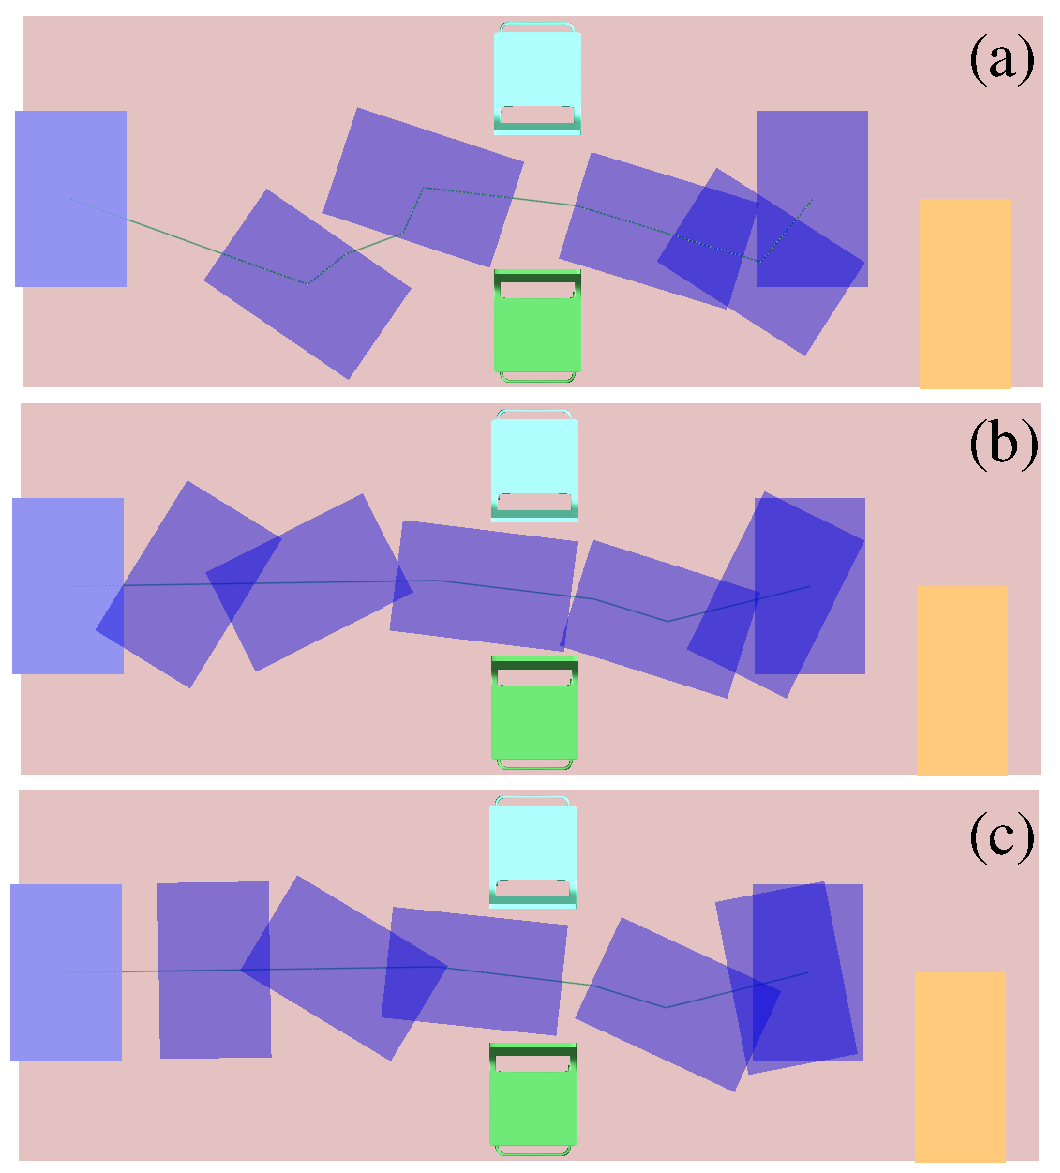
\includegraphics[width = 0.8\linewidth]
        {src/chap1-path-optimization/bb-plan-optim.pdf}}
      \caption{Top view: (a) RRT-Connect path for the bounding box
        passing between two chairs. (b) Optimized bounding box path by
        random optimization (RO). (c) Optimized bounding box after
        adding regular sampling optimization (RSO) .}
      \label{fig:chap1-bb-plan-optim}
\end{figure}

Assuming full knowledge of the environment, the RRT algorithm produces
a collision-free piecewise linear path $P_{RRT}$ for the robot
bounding box (in offline mode), i.e. the path consists of the
concatenation of linear local paths $LP_{RRT}$.

Due to the probabilistic nature of RRT, $P_{RRT}$ may not be optimal
in terms of length, and a preliminary random shortcut optimization
(RO) can be run in order to shorten it (See
\autoref{fig:chap1-bb-plan-optim}). While the optimized path $P$ is
collision-free, the bounding box orientation is such that it could
lead to an unrealistic trajectory that is not time-optimal. For
instance, the humanoid robot could spend a long time walking sideways
or backwards over a long distance in an open space. An additional
optimization stage is introduced to address this issue in the next
section.

\subsection{Bounding Box Path Optimization}
Note that each configuration \config{} can be written as $q =
(\mathbf{X},~\theta)$, where $\mathbf{X} = (x,~y)$ describes the
bounding box position in the horizontal plane, and $\theta$ gives its
orientation.  The optimizer reorients the bounding box along $P$ by
changing $\theta$ while retaining the value of $\mathbf{X}$.

For this purpose, an A$^{*}$ search algorithm is executed; first $P$ is
regularly sampled. Using a discrete set of possible orientations for
each sample configuration and an adequate heuristic estimation
function, the bounding box orientation is then modified along $P$. An
optimized path $P_{opt}$ is created and leads to a realistic
time-optimal trajectory.

\subsubsection{Preliminary Notations}
After running RO on the piecewise linear path $P_{RRT}$, the
path $P$ is also piecewise linear, and its first and last
configurations are denoted by $q_s$ and $q_g$.

Let $d_{sample} \in \mathbb{R}_+^*$ be a sampling distance. Sampling
$P$ with a distance $d_{sample}$ means dividing each local path $LP_j$
of $P$ into smaller local paths of length $d_{sample}$; each new local
path end is a sample configuration. The $n^{th}$ sample configuration
of $P$ in its initial state can be obtained by indexing new local path
ends starting from $q_s$, and is denoted by $q_n^{init}$.

\begin{figure}
  \centering
      {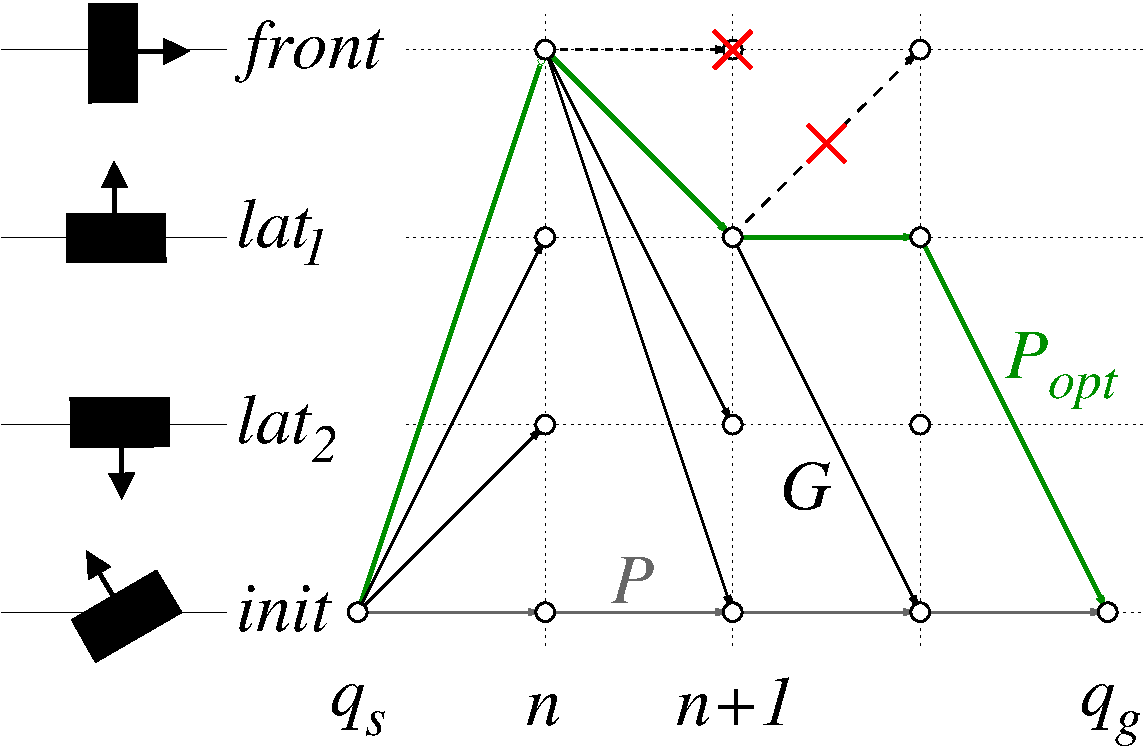
\includegraphics[width = 0.75\linewidth]
        {src/chap1-path-optimization/A-star.pdf}}
      \caption{Each initial sample configuration can be rotated and be
        in one of four states. Starting from $q_s$, the A$^{*}$ search
        algorithm searches the graph $G$ that contains only valid
        nodes and arcs to produce an optimized path $P_{opt}$.}
      \label{fig:chap1-A-star}
\end{figure}

The possible orientation states need to be defined. We aim to make a
humanoid robot reach its goal as soon as possible. Since the robot is
faster while walking straight than side-stepping, we attempt to change
the orientation of each initial sample configuration $q_n^{init}$ such
that the bounding box is tangent to the local path and introduce a new
configuration denoted by $q_n^{front}$. To take into account the fact
that there may be obstacles that forbid a frontal orientation, we also
create $q_n^{lat_1}$ and $q_n^{lat_2}$ that are rotated by
$\frac{\pi}{2}$ and $-\frac{\pi}{2}$ relative to the path tangent, see
\autoref{fig:chap1-A-star}. One particular case is local path end
configurations: the mean direction of the two adjacent local paths is
considered to define frontal and lateral configurations. This is done
to ensure a smooth transition between two local paths.

A sample configuration whose orientation is unknown will be denoted by
$q_n^{state}$. It can have any orientation state of the set
$\{init,~front,~lat_1,~lat_2\}$ except for $q_s$ and $q_g$ which
remain in their initial state.  Ideally, the algorithm should be able
(as long as there are no obstacles) to put each sample configuration
in the frontal state, create a new path $P_{opt}$ and generate a
time-optimal trajectory for the robot.

An A$^{*}$ search is run to achieve this goal; the algorithm functions are
described in the following section.

\subsubsection{A$^{*}$ Function Definition}
\label{sec:chap1-A-star}
An A$^{*}$ search algorithm can find an optimal path in a graph
as long as a graph and an evaluation function are correctly
defined. Starting from $q_s$, A$^{*}$ expands in each iteration the
possible transitions from one sample to the next one in the graph and
evaluates with the evaluation function the cost of going through each
different state, see \autoref{fig:chap1-A-star}.

A graph $G$ is defined to be a set of nodes and arcs. A valid node
$q_n^{state_n}$ is defined to be a configuration with no collisions,
and a valid arc $q_n^{state_n}q_{n+1}^{state_{n+1}}$ is a
collision-free local path. The whole graph $G$ could be built before
running A$^{*}$ by testing all nodes and arcs and making sure they are
collision-free. But collision tests are slow, and A$^{*}$ uses a heuristic
estimation function to avoid going through all nodes. An empty graph
$G$ is thus initialized and nodes and arcs are built only when
necessary. A successor operator needs to be defined for this purpose.

\begin{figure}
  \centering
      {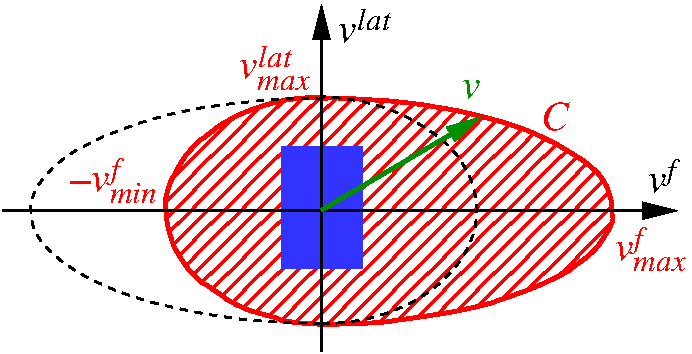
\includegraphics[width = 0.75\linewidth]
        {src/chap1-path-optimization/elliptic-constraint.pdf}}
      \caption{The rectangular bounding box speed vector $v$ is
        bounded inside the hashed area defined by the speed constraint
        $C$. The area is bounded by the union of two half-ellipsoids.}
      \label{fig:chap1-elliptic-constraint}
\end{figure}

\paragraph{The Successor operator $\Gamma(q_n^{state_n})$:}
Its value for any node $q_n^{state_n}$ is a set
$\{(q_{n+1}^{state_{n+1}},~c_{n,n+1})\}$, where
$q_{n+1}^{state_{n+1}}$ denotes a successor node, and $c_{n,n+1}$ is
the cost of going from $q_n^{state_n}$ to $q_{n+1}^{state_{n+1}}$. The
cost $c_{n,n+1}$ is defined to be the distance
$D(q_n^{state_n},~q_{n+1}^{state_{n+1}})$ between two nodes of $G$; it
computes the walk time from $q_n^{state_n}$ to
$q_{n+1}^{state_{n+1}}$. The speed constraint $C$ is defined as:
\begin{equation}
C = \left\{
\begin{array}{l l l}
  (\frac{v^{f}}{v_{max}^{f}})^2 +
  (\frac{v^{lat}}{v_{max}^{lat}})^2 - 1
  \quad \text{if } v^f >= 0 \\

  \\

  (\frac{v^{f}}{v_{min}^{f}})^2 +
  (\frac{v^{lat}}{v_{max}^{lat}})^2 - 1
  \quad \text{if } v^f < 0
\end{array} \right.
\end{equation}
where $v^{f}$ and $v^{lat}$ are respectively the frontal and lateral
speed, and $v_{min}^f$ $v_{max}^{f}$ and $v_{max}^{lat}$ their minimum
and maximum values (See
\autoref{fig:chap1-elliptic-constraint}). $D(q_n^{state_n},~q_{n+1}^{state_{n+1}})$
can be then computed by integrating this speed constraint along it.

Having expressed the successor operator, which allows the optimizer to
choose which node to expand at each iteration, the A$^{*}$ evaluation
function can be defined.

\paragraph{The Evaluation Function $\hat{f}(q_n^{state})$:}
It is the estimated cost of an optimal path going through
$q_n^{state}$ from $q_s$ to $q_g$ and can be written as:
\begin{equation}
  \hat{f}(q_n^{state}) = \hat{g}(q_n^{state}) + \hat{h}(q_n^{state})
\end{equation}
where $\hat{g}(q_n^{state})$ is the estimated cost of the optimal path
from $q_s$ to $q_n^{state}$ and $\hat{h}(q_n^{state})$ is a heuristic
function giving the estimated cost of the optimal path from
$q_n^{state}$ to $q_g$.

$\hat{h}(q_n^{state})$ must verify $\hat{h}(q_n^{state}) \leq
h(q_n^{state})$ to ensure that the algorithm is admissible, i.e. the
path from $q_s$ to $q_g$ is optimal. Since the robot is fastest while
walking straight forward in the absence of obstacles,
$\hat{h}(q_n^{state})$ is defined as:
\begin{equation}
  \begin{split}
  \hat{h}(q_n^{state}) &= D(q_n^{state},~q_{n+1}^{front}) \\
  &+ \sum_{k=1}^{N_{sample}-n-2} D(q_{n+k}^{front},~q_{n+k+1}^{front}) \\
  &+ D(q_{n+1}^{front},~q_g)
  \end{split}
\end{equation}
where $N_{sample}$ is the total number of initial sample
configurations in $P$ including $q_s$ and
$q_g$. $\hat{h}(q_n^{state})$ thus sums the cost of walking along $P$
while staying tangential to the path with the start and
end transition costs from $q_n^{state}$ and to $q_g$.

Now that the A$^{*}$ functions are fully defined, a search algorithm can be
run to compute an optimal path $P_{opt}$ by changing the orientation
of each sample node. An example is shown in
\autoref{fig:chap1-hash-direct-path}.

\begin{figure}
  \centering
      {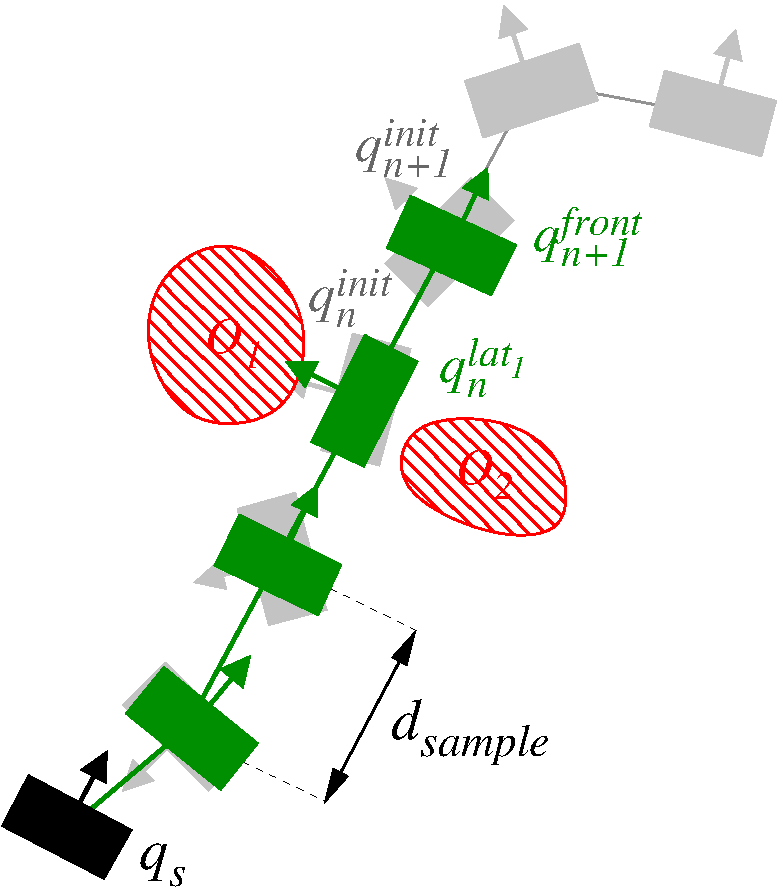
\includegraphics[width = 0.75\linewidth]
        {src/chap1-path-optimization/hash-direct-path.pdf}}
      \caption{Local paths are regularly sampled (light grey) and each
        sample configuration is reoriented (dark) while considering
        obstacles $O_1$ and $O_2$.}
      \label{fig:chap1-hash-direct-path}
\end{figure}

\subsection{Motion Generation for a Humanoid Robot}

A collision-free path $P$ for the 3-DoF bounding box can be found
using RRT-Connect and RO. The regular sampling optimization (RSO),
which is the subject of this paper, is then applied on the path and
produces a path $P_{opt}$ that gives priority to nonholonomic motion.

Once the bounding box trajectory is computed, the robot has to walk
along it. A footstep sequence is thus generated along $P_{opt}$ by
geometric decomposition of the path, and the pattern generator cited
in \autoref{sec:chap1-humanoid-walk-planning} then produces the robot
whole-body trajectory.

\section{Examples}
\label{sec:chap1-examples}

\begin{table}
\centering
\begin{tabular}{c|c|c|c|c|c|}
  \cline{2-6}
  & RRT-Connect & RO & RSO & Robot Trajectory & Total\\
  \hline
  \multicolumn{1}{|c|}{Chairs} & $3.97$ & $1.89$ & $2.14$ & $66.1$ & $74.1$\\
  \hline
  \multicolumn{1}{|c|}{Boxes} & $0.0917$ & $2.50$ & $0.238$ & $65.7$ & $68.6$\\
  \hline
  \multicolumn{1}{|c|}{Apartment} & $1.21$ & $2.43$ & $2.41$ & $223$ & $229$ \\
  \hline
\end{tabular}
\caption{Computational time (s) of each planning stage for the
  presented scenarios.}
\label{tab:chap1-computation-time}
\end{table}

\begin{table}
\centering
\begin{tabular}{c|c|c|}
  \cline{2-3}
  & RO & RO+RSO \\
  \hline
  \multicolumn{1}{|c|}{Chairs} & $40$ & $35$ \\
  \hline
  \multicolumn{1}{|c|}{Boxes} & $66$ & $57$ \\
  \hline
  \multicolumn{1}{|c|}{Apartment} & $200$ & $120$ \\
  \hline
\end{tabular}
\caption{Humanoid robot walk time (s) for the presented scenarios
  using RO alone and a RO-RSO combination.}
\label{tab:chap1-walk-time}
\end{table}

\begin{figure}
  \centering
      {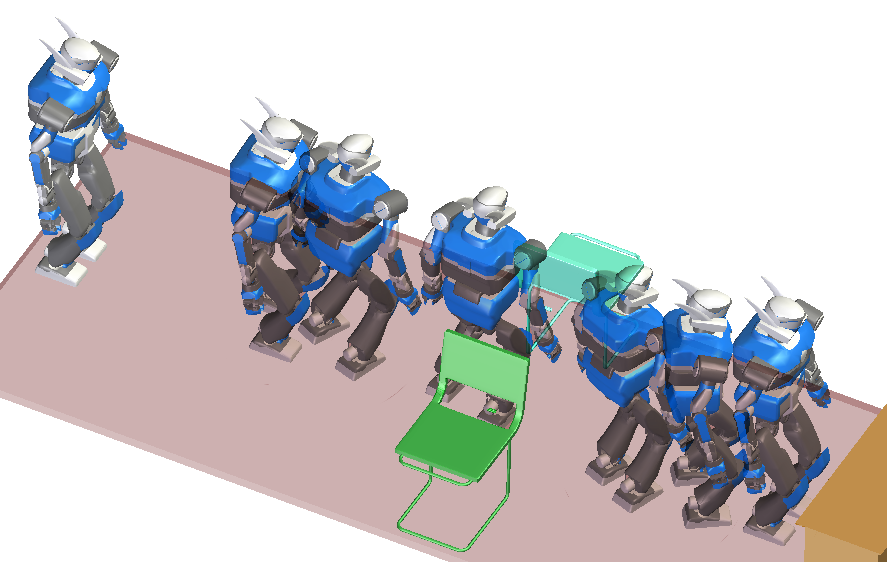
\includegraphics[width = \linewidth]
        {src/chap1-path-optimization/chairs-hash-optim-perspective-hrp2.png}}
      \caption{Perspective view of the simulated HRP-2 trajectory on
        the final optimized path passing between two chairs.}
      \label{fig:chap1-chairs-hash-optim-perspective-hrp2}
\end{figure}

This section presents experimental results of the path optimizer after
it has been inserted in the previously described walk planning
scheme. Distance parameters $v_{max}^f$, $v_{max}^{lat}$, $v_{min}^f$
are set to 0.5, 0.1, and 0.25 respectively. Note that these parameters
give an idea of the robot walking speed and play a key role in giving
priority to forward walking with respect to lateral and backwards
walking, but do not hold any physical significance, hence the absence
of units.

Since the A$^{*}$ search only takes place over the graph of discretized
configurations of the input path. It is important to choose a proper
value of the sampling interval $d_{sample}$. If the value is too
small, the search space will be much bigger, possibly leading to
better trajectories, but leading to an explosion of the A$^{*}$ search
time. If the value is too high, the A$^{*}$ search will be very fast in the
small trajectory space, but we risk missing some optimizations on the
trajectory. We found that setting $d_{sample}$ to be equal to
$\frac{h}{6}$, where $h$ is the humanoid height provided a good
comprise between computation time and trajectory quality: $d_{sample}$
is then a broad approximation of the nominal human step length.

Tests are performed on a 2.13 GHz Intel Core 2 Duo PC with 2 GB RAM.
Simulations of the humanoid robot HRP-2 are run in three scenarios.
The first one is a small environment where HRP-2 has to pass between
two chairs. The second environment is uncluttered with few obstacles
lying around, while the last one is a bigger apartment environment
where the robot has to move from one room to another while passing
through doors. The chairs scenario motion is also replayed on the real
robot HRP-2 (See Figure \ref{fig:chap1-hrp2-chairs}).

\begin{figure}
  \centering{
    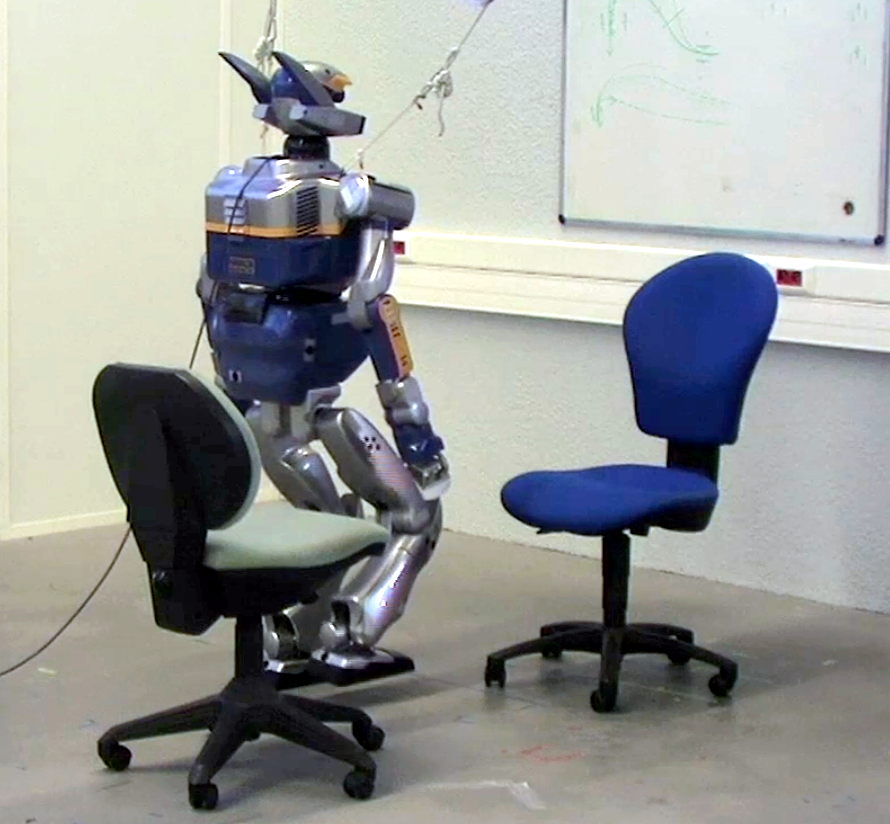
\includegraphics[width = 0.75\linewidth]
                    {src/chap1-path-optimization/hrp2-chairs.png}}
  \caption{Humanoid Robot HRP-2 uses holonomic motion, or
    side-stepping, to pass between two chairs.}
  \label{fig:chap1-hrp2-chairs}
\end{figure}

\ref{tab:chap1-computation-time} shows computation times for each
stage of the planning scheme: RRT-Connect, RO, RSO, and the whole-body
robot trajectory generation. In order to show the optimizer
contribution, robot walk times are also measured by creating a
trajectory directly after RO, and comparing it with a trajectory where
the RSO was added, see \autoref{tab:chap1-walk-time}.

\subsection{``Chairs'' Scenario}
\label{subsec:chap1-chairs}

\autoref{fig:chap1-bb-plan-optim} shows the bounding box RRT path
and the RO path for the chairs scenario. It is obvious that RO creates
a shorter path, but the bounding box starts rotating from the
beginning of the path even though the two chairs are still far. This
causes the robot trajectory to be unrealistic on one hand and, since
walking sideways takes a longer time than walking straight, to also
not be time-optimal.

\begin{figure}
  \centering
      {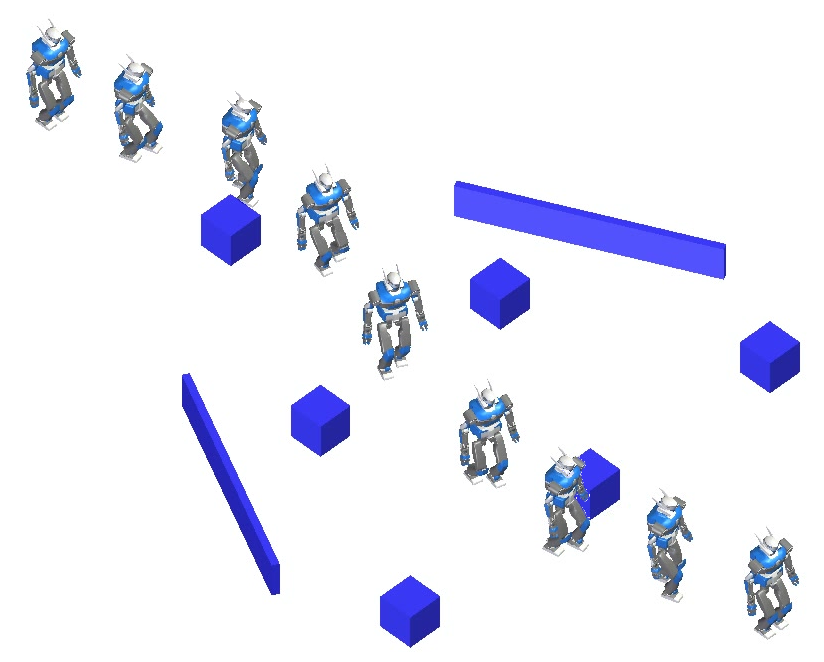
\includegraphics[width = \linewidth]
        {src/chap1-path-optimization/galton-hash-optim-perspective-hrp2.png}}
      \caption{Perspective view of HRP-2 optimized trajectory in the
        Galton board scenario.}
      \label{fig:chap1-galton-hash-optim-perspective-hrp2}
\end{figure}

However, after applying RSO, it is clear that the bounding box stays
oriented towards the front and rotates only when it reaches the
chairs. \autoref{fig:chap1-chairs-hash-optim-perspective-hrp2} and
\autoref{tab:chap1-walk-time} show that the walk time is shorter by 5
s and the final trajectory for HRP-2 is more realistic. Note that the
RSO takes 2,144 ms to be executed on the chairs path, which is less
than 3\% of the total computation time.

\subsection{``Galton'' Scenario}
An uncluttered environment is considered in this case, and
it can be seen that RRT-Connect and RSO computation times are very low
compared to other environments. This can be explained by the fact that
a tree connecting start and goal configurations is easier to find, and
that the frontal orientation state is valid for all considered samples
on the path (See \autoref{fig:chap1-galton-hash-optim-perspective-hrp2}).

\subsection{``Apartment'' Scenario}
The planning scheme is finally applied in the apartment scenario. In
\autoref{fig:chap1-apartment-hash-optim-perspective-hrp2}, it is
evident that HRP-2 walks facing forward through the doors. As with
previous scenarios, the trajectory is more realistic than a trajectory
where RSO is not used. The added computation time for RSO is 2,412 ms,
which is insignificant compared to the 228 s it takes for the whole
planning scheme.

Additionally, since the environment is significantly larger and more
constrained than the previous ones, the walk time difference is more
striking: \autoref{tab:chap1-walk-time} shows that it takes the robot
80 s less to cross the apartment when an RO-RSO combination is used.

\begin{figure}
  \centering
      {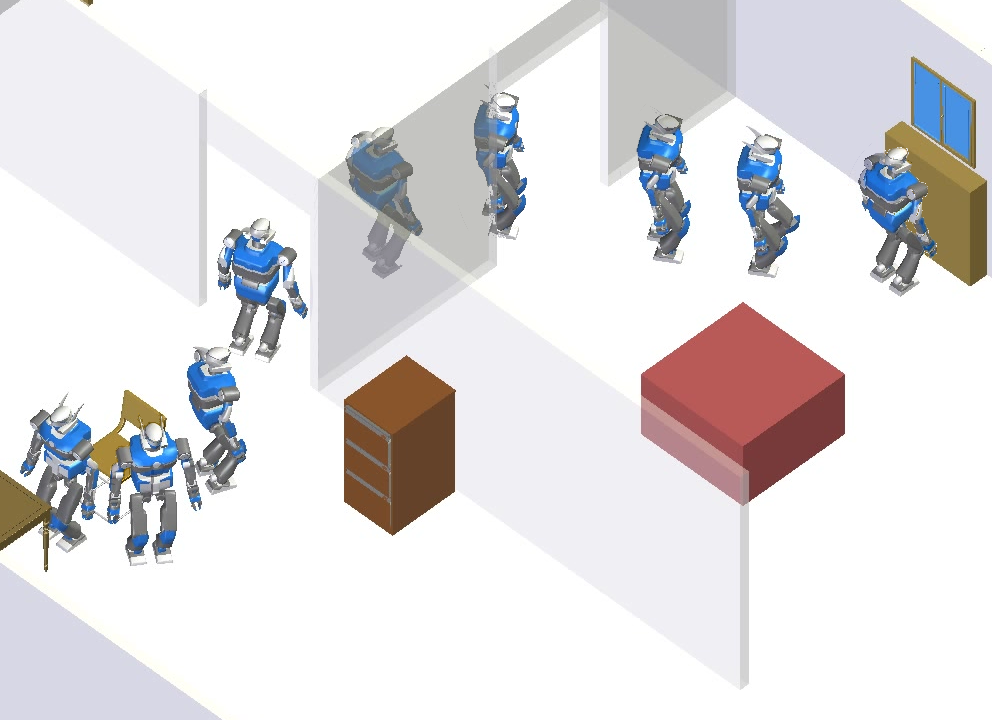
\includegraphics[width = \linewidth]
        {src/chap1-path-optimization/apartment-hash-optim-perspective-hrp2.png}}
      \caption{Perspective view of HRP-2 optimized trajectory in the
        apartment scenario.}
      \label{fig:chap1-apartment-hash-optim-perspective-hrp2}
\end{figure}

\section{Conclusion}
In this chapter, a novel simple optimization method is
presented for humanoid walk planning that relies on a decoupling
between trajectory and robot orientations. It uses an A$^{*}$ search that
takes as input a path for the robot bounding box, and produces a path
where a discrete set of configurations have been reoriented to generate
a realistic time-optimal walk trajectory. Results show that new
trajectories are more satisfactory while the added computation time is
insignificant compared to the whole planning time.

This approach can be used in other fields such as graphical animation
for digital actors to adapt the body orientation with respect to the
goal during locomotion. With a motion capture library containing
prerecorded nonholonomic and holonomic walk behaviors, it is possible
to lay this behavior on the actor trajectory and produce realistic
movements.

Achieving humanoid walk planning using the bounding box approach is
both simple and efficient; it allows using off-the shelf
sampling-based planners to efficiently explore the configurations
space, thus removing the need to take into account additional
kinematic and balance constraints when planning for the whole
articulated robot. But it has one major drawback: in order to have a
sound framework which always produces collision-free walking
trajectories, the bounding box must contain all the robot geometries
and take into account the robot swaying motion during walking. It is
thus a rather conservative method, and it might not succeed in finding
collision-free trajectories in cluttered environments. If we go back
to the chairs example in \ref{subsec:chap1-chairs}, we can show that
the lateral walking motion could have been avoided if the HRP-2 lifted
its arms over the two chairs. Besides leading to an even faster
motion, walking forward could be necessary if vision systems were
needed to achieve robot localization and/or environment mapping.

In the next chapter, we introduce a sound whole-body motion planning
algorithm that allows planning collision-free walking trajectories for
the fully articulated humanoid robot, hence releasing it from its
bounding box constraint and increasing its accessible workspace.


%% \backmatter

%% \addcontentsline{toc}{chapter}{Liste of figures}
%% \listoffigures
%% \addcontentsline{toc}{chapter}{Liste of tables}
%% \listoftables

%
% Bibliography
\begin{singlespace}
\addcontentsline{toc}{chapter}{Bibliography}
\bibliography{thesis}
%
% Index
%% \cleardoublepage
%% \addcontentsline{toc}{chapter}{Index}
%% \printindex
\end{singlespace}
%
\end{document}
